\documentclass[tufte-handout]{standalone}
\usepackage{mathpazo} % Sets Palatino as the main font
\usepackage{tikz}
\usetikzlibrary{3d, angles, quotes, calc, backgrounds}
\usetikzlibrary{decorations.markings}
\begin{document}
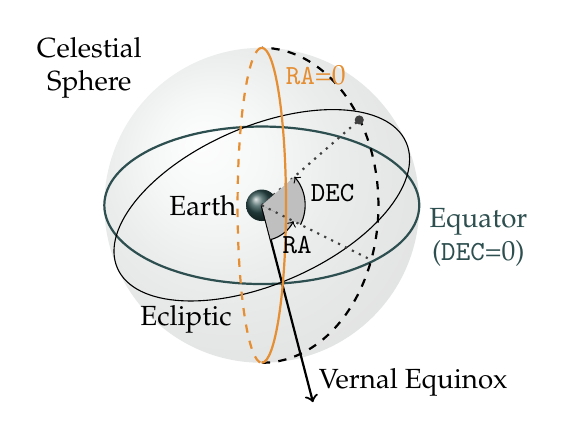
\begin{tikzpicture}[scale=2]

   %my colors
\definecolor{darkslategray}{rgb}{0.18, 0.31, 0.31}
\definecolor{myorange}{rgb}{0.89804, 0.55686, 0.19608}



    % Define radius of the celestial sphere and the Earth
    \def\R{1} % Radius of the celestial sphere
    \def\r{0.1} % Radius of the Earth

    % Draw the celestial sphere
    \shade[ball color=darkslategray!40!white,opacity=0.15] (0,0) circle (\R); % semi-transparent sphere
    \node[anchor=east, xshift=0.6cm, yshift=-0.25cm, align=center] at (-\R,\R) {Celestial \\ Sphere};

    % Draw the Earth at the center
    \shade[ball color=darkslategray] (0,0) circle (\r); % Earth
    \node[anchor=east, xshift=-0.4cm] at (\r,0) {{Earth}};

    \draw[->, thick, black] (0, 0) -- (0.325, -1.25);
    \node[black, anchor=west, yshift=-0.25cm, xshift=0.4cm] at (\r,-\R) {Vernal Equinox};

    % Equator and ecliptic
    \draw[thick, darkslategray, rotate around={0:(0,0)}] (0,0) ellipse (\R{} and \R/2);  % Equator
    \node[darkslategray,anchor=south, yshift=-0.9cm, xshift=0.75cm, align=center] at (\R,0) {Equator \\ (\texttt{DEC}=0)};
    \draw[rotate around={23.5:(0,0)}] (0,0) ellipse (\R{} and \R/2); % Ecliptic
    \node[rotate=0,anchor=south, xshift=-80, yshift=-1.75cm] at (\R-0.075,0) {{Ecliptic}};
    % Right Ascension and Declination lines for the source
    \pgfmathsetmacro{\RAangle}{70} % Right Ascension in degrees
    \pgfmathsetmacro{\Decangle}{40} % Declination in degrees

    % Convert spherical to Cartesian coordinates
    \pgfmathsetmacro{\x}{\R * cos(\Decangle) * cos(\RAangle)}
    \pgfmathsetmacro{\y}{\R * cos(\Decangle) * sin(\RAangle)}
    \pgfmathsetmacro{\z}{\R * sin(\Decangle)}

    % Draw RA line (projected on the equatorial plane)
    \draw[thick, dashed] (0,-\R) arc (-90:90:\R/1.35 and \R);
    \draw[thick,dotted,darkgray] (0,0) -- (\y,\z,\x);
    
    \coordinate (vernal_eq) at (0.325, -1.25);
    \coordinate (ra) at (0.7,-0.35);
    \coordinate (dec) at (\y,\z,\x);
    \coordinate (O) at (0, 0);
    \pic[draw, ->, angle eccentricity=1.2, angle radius=0.45cm, color = black,fill =lightgray] {angle = vernal_eq--O--ra};
    

    \pic[draw, ->, angle eccentricity=1.2, angle radius=0.55cm, color = black,fill =lightgray] {angle = ra--O--dec};
    \node[black] at ($(O)+(0.45,0.075)$) {{\texttt{DEC}}};

    \draw[thick,dotted,darkgray] (0,0) -- (0.7,-0.35); 

     % zero RA 
    \draw[thick, myorange] (0,-\R) arc (-90:90:\R/6.5 and \R);
    \draw[thick, myorange, dashed] (0,\R) arc (90:270:\R/6.5 and \R);
    \node[myorange, anchor=west, xshift=-0.5, yshift=-0.35cm] at (\r,\R) {{\texttt{RA}=0}};
    \node[black] at ($(O)+(0.225,-0.25)$) {{\texttt{RA}}};
    
    % Source point
    \filldraw[darkgray] (\y,\z,\x) circle (0.025cm);
    
\end{tikzpicture}
\end{document}